\documentclass[12pt,reqno, twoside]{amsbook}
%%%%%%%%%%%%%%%%%%%%%%%%%%%%%%%%%%%%%%%%%%%%%%%%%%%%%%%%%%%%%%%%%%%%%%%%%%%%%%%%%%%%%%%%%%%%%%%%%%%%%%%%%%%%%%%%%%%%%%%%%%%%%%%%%%%%%%%%%%%%%%%%%%%%%%%%%%%%%%%%%%%%%%%%%%%%%%%%%%%%%%%%%%%%%%%%%%%%%%%%%%%%%%%%%%%%%%%%%%%%%%%%%%%%%%%%%%%%%%%%%%%%%%%%%%%%
\usepackage{eurosym}
\usepackage{amsmath}
\usepackage{amssymb}
\usepackage{amsfonts}
\usepackage[onehalfspacing]{setspace}
\usepackage{chngcntr}
\usepackage{graphicx}
\usepackage[a4paper, margin=2.5cm]{geometry}
\usepackage[english]{babel}
\usepackage{fancyhdr}
\usepackage{titlesec}
\usepackage{enumitem}
\usepackage{etoolbox}
\usepackage{comment}
\usepackage{caption}
\usepackage{enumitem}
\usepackage{float}
% you may need to uncomment the command below if you use eps format for figures
%\usepackage{epstopdf}

\makeatletter
\def
\section{\@startsection{section}{1}%
  \z@{.5\linespacing\@plus.7\linespacing}{.25\linespacing}%
{\normalfont\bfseries\flushleft}}
\def
\subsection{\@startsection{subsection}{2}%
  \z@{.5\linespacing\@plus.7\linespacing}{.25\linespacing}%
{\normalfont\bfseries\flushleft}}

\makeatother
\setcounter{MaxMatrixCols}{10}

\providecommand{\U}[1]{\protect\rule{.1in}{.1in}}
\theoremstyle{plain}
\newtheorem{acknowledgement}{Acknowledgement}
\newtheorem{algorithm}{Algorithm}[chapter]
\newtheorem{axiom}{Axiom}[chapter]
\newtheorem{case}{Case}[chapter]
\newtheorem{claim}{Claim}[chapter]
\newtheorem{conclusion}{Conclusion}[chapter]
\newtheorem{condition}{Condition}[chapter]
\newtheorem{conjecture}{Conjecture}[chapter]
\newtheorem{corollary}{Corollary}[chapter]
\newtheorem{criterion}{Criterion}[chapter]
\newtheorem{definition}{Definition}[chapter]
\newtheorem{example}{Example}[chapter]
\newtheorem{exercise}{Exercise}[chapter]
\newtheorem{lemma}{Lemma}[chapter]
\newtheorem{notation}{Notation}[chapter]
\newtheorem{problem}{Problem}[chapter]
\newtheorem{proposition}{Proposition}[chapter]
\newtheorem{remark}{Remark}[chapter]
\newtheorem{solution}{Solution}[chapter]
\newtheorem{summary}{Summary}[chapter]
\newtheorem{theorem}{Theorem}[chapter]
\numberwithin{equation}{chapter}

% Please write the references according to your school

\newenvironment{dedication}
{%\clearpage           % we want a new page
  \thispagestyle{empty}% no header and footer
  \vspace*{\stretch{1}}% some space at the top
  \itshape             % the text is in italics
  \raggedleft          % flush to the right margin
}
{\par % end the paragraph
  \vspace{\stretch{3}} % space at bottom is three times that at the top
  %\clearpage           % finish off the page
}
\numberwithin{section}{chapter}
\fancyhead{}
\fancyfoot{}
\pagestyle{fancy}
\fancyfoot[LE,RO]{\thepage}

\makeatletter
\def\ps@plain{\ps@empty
  \def\@evenfoot{%
    \normalfont\scriptsize
    \rlap{\thepage}\hfil
  }%
  \def\@oddfoot{%
    \normalfont\scriptsize \hfil
  \llap{\thepage}}%
}
\makeatother
\renewcommand{\headrulewidth}{0pt}
\renewcommand{\footrulewidth}{0pt}

\begin{document}
\frontmatter
\addtocontents{toc}{\setcounter{tocdepth}{2}}
\thispagestyle{empty}

\begin{dedication}%

  \begin{flushright}
    \textit{Write here your dedication!}
  \end{flushright}%
\end{dedication}

\setcounter{page}{1}
\pagenumbering{roman} %
\chapter*{Cover}

\chapter*{Acknowledgment}

Write here the acknowledgments and grants, if any

\chapter*{Resumo}

Write here your abstract in Portuguese

\chapter*{Abstract}

Write here your abstract in English

\tableofcontents

\mainmatter
\setcounter{page}{1} \pagenumbering{arabic}

\chapter{Introduction}
\section{Background \& Context}
\noindent The landscape of higher education has undergone significant transformation through the widespread adoption of digital technologies and learning management systems. This digital evolution has created unprecendented opportunities for institutions to leverage data analytics and innovative pegagogical approaches in order to enhance student learning outcomes and insitutional effectiveness. Within this context, the integration of gamification principles with educational analytics represents a promising avenue for addressing persistent challenges in student engagement, motivation and academic performance monitoring.

The concept of gamification, defined as the application of game design elements
in non-game contexts~\cite{deterding_gamification_2011}, has gained
considerable traction in educational settings as a mechanism for increasing
student motivation and engagement. When combined with learning analytics, which
involves the measurement, collection, analysis and reporting of data about
students and their contexts for purposes of understanding and optimizing
learning, gamification can prove to be a powerful tool for both students and
teachers, both to monitor and improve the learning process.

The Learning Scorecard perfectly exemplifies this convergence of gamification
and educational analytics. Originally conceived as a comprehensive academic
performance management system, the LS has evolved through multiple iterations
to become a sophisticated platform that merges business intelligence
methodologies with educational gamification strategies. The platform's core
objective is to provide the students and faculty with actionable insights into
the learning progress while maintaining high levels of student engagement
through game-like mechanics.

However, the evolution of the Learning Scorecard has revealed, throughout the
years, significant architectural and operational limitations that constrain its
effectiveness and adoption within institutional contexts. These limitations,
particularly regarding system integration, data collection efficiency and user
accessibility, have urged a fundamental reconceptualization of the platform's
technical infrastructure and deployment strategy.

\section{Statement of the Problem}
\noindent The current implementation of the Learning Scorecard (version 2.0) platform presents several critical challenges that prevent its effectiveness and widespread adoption within higher education institutions. These challenges can be categorized into three primary domains: technical architecture, operational efficiency and institutional integration.

The existing Learning Scorecard operates as a standalone web application with
external infrastructure dependencies, including cloud-hosted databases and
third party service integrations. This architectural approach creates several
complications: first, it requires a separate authentication system and user
management processes that exist parallel to institutional systems; second, it
requires ongoing maintenance of external infrastructure, increasing operational
costs and security vulnerabilities; third, it creates data silos, isolated
collections of data that prevent seamless integration and data sharing with
existing institutional learning management systems.

The current system requires substancial manual data entry from both students
and faculty in order to populate the platform with the necessary academic and
performance information. This manual input requirement creates multiple
friction points: Students must duplicate the effort of entering information
that already exists in institutional systems; faculty members face additional
administrative burdens in maintaining accurate records of data across multiple
platforms; the potential for data inconsistencies and errors increases
significantly due to human input mistakes.

Perhaps most critically, the standalone nature of the current Learning
Scorecard creates barriers to institutional adoption and sustained usage.
Students and faculty must actively choose to visit the external platform,
creating an additional step in their academic workflow. The platform lacks
integration with existing institutional systems, perventing it from leveraging
the data already collected through learning management systems like Moodle.

These challenges collectively result in a reduced user adoption, increased
maintenance costs, compromised data accuracy and limited institutional support
for the platform's continued development and deployment.

\section{Aims and Objectives}
\noindent This thesis addresses the identified limitations through the development and evaluation of a Learning Scorecard version 2.5, which fundamentally reconceptualizes the platform's architecture and deployment strategy. The objectives are structured around both technical innovation and empirical validation of the proposed solution.

From a technical perspective, this thesis aims to: (1) design and implement a
modular plugin architecture that could seamlessly integrate with ISCTE's Moodle
infrastructure; (2) develop automated data collection mechanism that leverage
Moodle's comprehensive student activity and performance data; (3) create user
interfaces that maintain consistency with Moodle's design patterns while
providing functionality of the Learning Scorecard platform; (4) ensure data
security and privacy protection through adherence to Moodle's established
security frameworks.

This thesis also seeks to validate the effectiveness of the integrated approach
through: (1) demonstration of reduced manual input requirements compared to
previous Learning Scorecard versions; (2) evaluation of user experience
improvements resulting from seamless integration with existing academic
workflows; (3) assessment of system performance and scalability within the
Moodle environment; (4) analysis of the platform's potential for broader
institutional adoption given its integration with existing infrastruture.

Beyond technical and empirical considerations, this thesis aims to contribute
to the broader understanding of how gamification platforms can be effectively
integrated within established educational technology ecosystems. The findings
will provide insights into best practices for developing educational technology
solutions that complement rather than compete with existing institutional
systems.
\section{Methodological Approach}
This thesis employs a design science methodology, combining systematic design
and development processes with empirical evaluation. The methodology
encompasses three primary phases: analysis and design, implementation and
development and evaluation and validation.

\textit{Analysis and Design Phase} The initial phase involves a comprehensive analysis of existing Learning Scorecard implementations, detailed examination of Moodle's plugin architecture and Service API capabilities and systematic requirements gathering. This phase includes mapping the Learning Scorecard concepts to Moodle's existing data structures and functionality, identifying integration opportunities and constraints and developing a comprehensive system architecture that addresses the identified limitations while preserving core platform capabilities.

\textit{Implementation and Development Phase} The development phase follows an agile methodology with iterative development cycles focused on delivering functional components that can be tested and refined throughout the process. The development approach emphasizes modular design and adherence to Moodle coding standards to ensure compatibility with Moodle's ecosystem. Key deliverables include a block plugin to exemplify a user interface component of the student interface and a local plugin for main functionality and who's responsible for the addition of database schemas that integrate with Moodle's existing data structures.

\textit{Evaluation and Validation Phase}
\section{Structure of the Thesis}
\noindent This thesis is organized into seven chapters that systematically address the objectives and present the development, implementation and evaluation of Learning Scorecard 2.5.

\textit{Chapter 2: Literature Review} provides comprehensive background on learning management systems, with particular focus on Moodle's architecture and capabilities and examines the theoretical foundations and practical applications of gamification in educational contexts. This chapter establishes the theoretical framework that suplements the design decisions throughout the thesis.

\textit{Chapter 3: The Learning Scorecard: Concept and Evolution} traces the historical development of the Learning Scorecard platform through its various iterations, analyzing the lessons learned from previous implementations and establishing the conceptual framework of the Learning Scorecard.

\textit{Chapter 4: System Architecture and Design} presents the technical architecture of the Learning Scorecard 2.5, including detailed requirements analysis, system design decisions, plugin architecture specification and database design. It's also presented a detailed mapping of Learning Scorecard concept to Moodle's existing functionality and its mapping feasibility. This chapter provides the technical foundation for understanding the implementation approach and design rationale.

\textit{Chapter 5: MVP} describes the key deliverables and presents the proposed solution and serves as a demonstration of some functionality from the Learning Scorecard and its feasibility as Moodle integrated plugins.

\textit{Chapter 6: Evaluation and Results}

\textit{Chapter 7: Conclusions}

\chapter{Literature Review}
\section{Learning Management Systems}
\noindent Learning Management Systems (LMS) represent sophisticated software applications engineered to administer, track, report, automate and deliver educational courses, training programs and comprehensive learning materials. Following their initial emergence in the late 1990s, these platforms have achieved near-universal adoption across higher education institutions globally. Recently, the unprecedented expansion of LMS usage has been significantly accelerated by the institutional shift toward remote learning by the COVID-19 pandemic.

There are a plethora of LMS available for educational institutions, with
ommercial and open-source platforms representing the two primary categories of
LMS offerings~\cite{mohd_kasim_choosing_2016}. Commercial LMS are either
available in the market for a price or, although very rarely, proprietary and
developped by the institution. In contrast, the open source alternative is
available at no cost to the institution, although technical expertise is
required aswell as regular functional assessments. Open-source systems provide
publicly accessible source code that institutions can modify and improve to
meet their specific requirements and needs \cite{cavus_comparison_2014}.

Moodle (Modular Object-Oriented Dynamic Learning Environment) stands as one of
the most widely adopted open-source learning management systems globally.
According to a recent systematic review on tendencies in the use of LMS, Moodle
is the most popular and preferred open-source
LMS~\cite{altinpulluk_systematic_2021}. The platform's extensive reach is
evidenced by its current deployment across 238 countries, serving approximately
468 million users worldwide~\cite{moodle_stats_2025}.

From a technical perspective, Moodle is built on a layered architecture that
ensures flexibility and scalability. The presentation layer handles the user
interface and allows users to interact both on desktop and mobile devices. The
application layer accommodates core functionalities and acts as an intermediary
between the presentation and data layer, supporting the installation of plugins
and modules to customize features. The data layer includes the database
management system, typically SQL-based, which stores and manages all the data.
This modular design allows institutions to customize the functionality and
appearance through a extensive plugin ecosystem.

\begin{figure}[H]
  \centering
  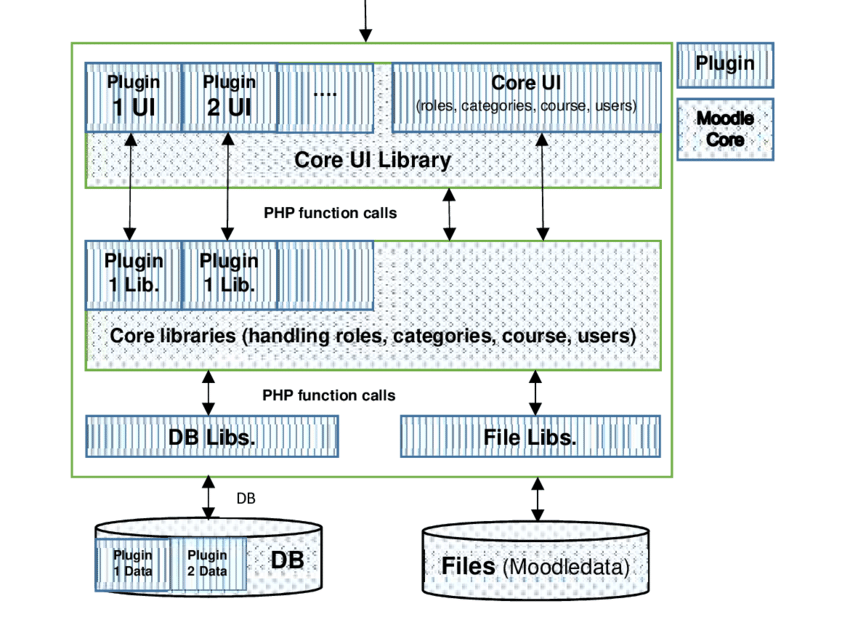
\includegraphics[width=0.8\textwidth]{images/Moodle-three-tier-architecture.png}
  \caption{Moodle three tier architecture. Source: Dolawattha et al.~\cite{dolawattha_impact_2019}.}
  \label{fig:moodle_arch}
\end{figure}

Moodle offers many plugins that allow for functionality expansion. There are
multiple types of plugins from local plugins, block plugins all the way to
antivirus plugins. Each with its own purpose and place in the moodle folder
structure.

\section{Gamification and Motivation in Education}
\subsection{Theoretical Perspectives on Gamification}
\subsection{Gamification and Student Engagement}

\chapter{The Learning Scorecard: Concept and Evolution}
\section{Genesis and Conceptualization of the Learning Scorecard}
\noindent The Learning Scorecard emerged from a fundamental pedagogical challenge identified within higher educational institutions: the lack of understanding by faculty members regarding the difficulties experienced by students in relations to the content taught in curricular units aswell as the students disinterest and lack motivation. Initially, this platform was conceptualized as a comprehensive academic performance management system designed to support both students and faculty through data-driven insights that assist teachers in continuously monitoring the curricular units they teach while enabling students to visualize their performance in each course in which they are enrolled. Their main mission was to offer higher education students an analytic environment that allows progress monitorization through a familiar game-like scope, contributing for a better learning experience.

The platform was originally conceptualized with three distinct user
perspectives: student view, teacher view and administrative view. The student
view provides essential visualizations that enable students to understand their
learning trajectory in a specific curricular unit while offering tools that
provide important data for continuous monitoring by faculty. The teacher view
provides management, evaluations and visualization tools for educators
regarding each curricular unit they teach, offering various visualizations to
track each students progress through all phases of the curricular unit along
with assessment tools.

\section{Evolution Through Iterative Development}
\subsection{Historical Overview of Versions}
\noindent The Learning Scorecard development began in the 2015/16 academic year as a collaborative project project undertaken by a group of Computer Science masters students enrolled in the Information Systems of Decision Support II curricular unit. This class established a foundation of rigorous analysis and systematic development that has characterized the platform's evolution throughout subsequent iterations.

The development timeline reflects the progression of features and refinements
with each major version addressing specific limitations and opportunities
identified through previous implementations. This iterative approach has
enabled the platform to evolve in response to changing technological
landscapes, pedagogical insights and institutional requirements while
maintaining consistency in core design principles.

\textbf{Learning Scorecard Version 1 (2016)}

\textbf{Learning Scorecard Version 2 (2017)}

\textbf{Learning Scorecard Version 3 (2018)}

\subsection{Lessons Learned from Prior Iterations}

The evolutionary development of the Learning Scorecard has yielded important
insights into the challenges and opportunities associated with educational
technology implementation in higher education contexts. These lessons has
directly informed the design decisions underlying Learning Scorecard 2.5 and
provide valuable guidance for future LS development efforts.

Previous iterations consistently revealed the critical importance of seamless
integration with existing institutional systems and workflows. Standalone
implementations, while providing flexibility and autonomy, created barries to
adoption through the requirement for separate authentication, manual data entry
and navigation between multiple platforms. These experiences highlighted the
need for deeper integration with institutional learning management systems to
achieve sustainable adoption and effectiveness.

Analysis of user behavior accross previous versions revealed important patterns
regarding the factors that drive sustained engagement with educational
technology platforms. Students demonstrated higher levels of engagement when
gamification elements were seamlessly integrated with existing academic
workflows rather than requiring separate platform visits or additional effort
investment. Faculty adoption correlated strongly with the availability of
actionable insights that directly supported pedagogical decision-making without
creating additional workload or administrative burden.

\textit{Scalability and Maintenance Considerations} The operational experience of maintaining standalone Learning Scorecard implementations revealed significant challenges related to infrastructure costs, security management and version compatibility. These experiences demonstrated the advantages of leveraging existing institutional infrastructure and support systems rather than maintaining separate technological stacks that require independent updates, security monitoring and user support.
\section{Learning Scorecard Conceptual Framework}

The Learning Scorecard (LS) conceptual framework encompasses a comprehensive
set of interconnected concepts designed to support gamified learning
experiences in higher education. This framework is organized around four
primary fomains that reflect different aspects of the educational experience:
Academic Structure and Organization, Gamification Mechanics, Social
LearningThese concepts can be organized into four primary domains: Academic
Structure, Gamification Mechanics, Social Learning and Recognition and
Achievement Systems. Each domain contains interconnected concepts that work
together to create a comprehensive educational technology ecosystem that
supports both individual learning, cooperation and institutional objectives.

\subsection{Academic Structure and Organization}

The academic foundation of the Learning Scorecard is built upon traditional
higher education organizational structures, adapted to support digital learning
environments.

\textbf{Courses and Curricular Units.} The system recognizes a two-tier academic structure where \textit{Courses} represent overarching academic programs (e.g., "Computer Science") that encompass multiple \textit{Curricular Units}. Each Curricular Unit corresponds to an individual subject with specific learning objectives, content and assessments that students must complete as part of their academic progression. This hierarchical organization maintains consistency with traditional academic frameworks while enabling digital tracking and gamification.

\textbf{Students and Faculty.} The system accommodates two primary user roles: \textit{Students}, who are enrolled in one or more Curricular Units and participate in gamified learning activities and \textit{Teachers} or Faculty members, who are responsible for creating and managing curricular content, designing learning activities and monitoring student progress within their assigned Curricular Units.

\textbf{Syllabus Contents, Calendar and Timeline.} \textit{Syllabus Contents} encompass all learning materials, resources and educational content within a Curricular Unit. The organizational framework includes both \textit{Calendar} and \textit{Timeline} concepts that serve as complementary planning systems, enabling students and faculty to organize learning activities and maintain temporal awareness of curricular progression.

\subsection{Gamification Mechanics}

The core gamification elements provide the foundation for student engagement
and progress tracking through game-like mechanics adapted to educational
contexts.

\textbf{Experience Points and Ranks.} \textit{Experience Points} (XP) serve as the fundamental currency of progress within the platform, earned through completion of various educational activities. The \textit{Rank} system establishes hierarchical progression levels based on accumulated XP, including ranks such as Newbie (entry level at 0 XP), Rookie, Skilled Expert, Master and Legendary. Faculty members can configure rank thresholds dynamically, with each rank unlocking new privileges and recognition within the platform.

\textbf{Quests.} \textit{Quests} represent the core educational activities that students complete to earn XP and demonstrate learning. The system categorizes quests into five distinct types: Class Attendance, Practical Assignment, Quiz, Exercise and Event. Each quest can be designated as mandatory (milestone quests) or optional, providing flexibility in curriculum design while maintaining educational objectives.

\textbf{Last Chances.} The \textit{Last Chance} mechanism provides opportunities for recovery and continued engagement when students fall behind or make mistakes, preventing permanent failure states that could lead to disengagement and ensuring continued participation throughout the academic term.

\subsection{Social Learning}

The social components of the Learning Scorecard foster collaboration and
healthy competition among students through structured group dynamics.

\textbf{Alliances.} \textit{Alliances} function as large-scale organizational units that typically correspond to academic classes or programs (e.g., LEI or ETI). These structures facilitate competition and comparison at the class level while maintaining educational coherence, enabling students to compare their progress through dedicated leaderboards and participate in alliance-specific activities.

\textbf{Guilds.} \textit{Guilds} represent smaller collaborative units within alliances, typically corresponding to project teams or study groups. The guild system promotes cooperative learning by encouraging mutual assistance among members, with guild-specific achievements, badges and leaderboards fostering team spirit while maintaining individual accountability within the collaborative framework.

\subsection{Recognition and Achievement System}

The recognition framework provides multiple pathways for acknowledging student
accomplishments and maintaining motivation through visible achievements.

\textbf{Badges.} The \textit{Badge} system provides targeted recognition for specific accomplishments and behaviors, featuring 39 different badges organized into four categories: individual achievements, guild-based accomplishments, forum participation and final questionnaire completion. Each category includes multiple tiers (bronze, silver, gold and platinum) corresponding to increasing levels of difficulty and commitment.

\textbf{Trophies.} \textit{Trophies} represent the highest level of achievement, awarded to top performers in various leaderboard categories including overall rankings (Best Score Player), guild performance (Best Guild) and combined metrics (Best Triathlon Player). Each trophy provides substantial XP rewards (typically 1000 XP) and serves as a highly visible symbol of excellence.

\textbf{Avatars.} The \textit{Avatar} system enables profile customization while serving as a visual indicator of progression. Students unlock new avatar options as they advance through rank levels, with both male and female options available at each tier, allowing for personal expression while maintaining the connection between visual representation and academic achievement.

\textbf{Leaderboards.} Multiple \textit{Leaderboard} systems enable various forms of competition and comparison through five distinct categories: overall individual rankings, guild-based comparisons, exercise-specific performance, quiz results and combined metrics. Each leaderboard displays position, username, rank, avatar and XP totals, creating transparency in academic performance while fostering healthy competition among participants.

\begin{comment}
\subsection{Monitoring and Analytics}

\subsubsection{Student Dashboard}
\paragraph\ The student dashboard serves as the central interface for progress monitoring and decision-making.
Students can view their advancement across different quest types, track XP accumulation, monitor rank progression and analyze their performance relative to peers.
The dashboard integrates all gamification elements into a cohesive user experience.

\subsubsection{History Tracking}
\paragraph\ The platform maintains comprehensive records of all student activities and achievements.
The history system allows students to review their XP gains from each quest, track their progression over time and understand the relationship between their efforts and outcomes.

\subsection{Faculty Management}

\subsubsection{Quest Configuration}
\paragraph\ Faculty members can create and manage quests through both individual interfaces and bulk Excel imports.
The system allows for dynamic quest addition throughout the term, enabling responsive curriculum adjustment based on student needs and learning objectives.

\subsubsection{Rank and XP Configuration}
\paragraph\ Instructors have comprehensive control over rank thresholds and XP distribution.
This flexibility enables adaptation to different course structures, student populations and learning objectives while maintaining game balance and engagement.

\subsection{Assessment Integration}

\subsubsection{Continuous Assessment Connection}
\paragraph\ The gamification system integrates directly with academic assessment, allowing XP and rank progression to contribute to final course grades.
This connection ensures that game mechanics support rather than distract from educational objectives.

\subsubsection{Difficulty and Challenge Scaling}
\paragraph\ The platform incorporates mechanisms for adjusting challenge levels and providing appropriate difficulty progression.
This ensures that all students can find appropriate challenges while maintaining engagement across diverse skill levels and learning paces.
\end{comment}

\chapter{System Architecture and Design}
\section{Requirements}
\noindent An imperative aspect in any application conceptualization is a thorough requirement analysis. These requirements can be functional (FR) or non functional (NFR) and shape the architectural decisions that are made during its development as well as assessing whether a system will succeed.

\textbf{Functional Requirements (FR)}

It's important to define what an engineer should strive for when determining
functional requirements as it will ultimately be what defines an application,
molds its functionality and consequently decides it's architecture. Functional
requirements are the essential characteristics that the system should deliver
that the end-user specifically demands.~\cite{saroja_functional_2023} A simpler
way to perceive it is that they define what the system should perform. It's
important with any version increment of the LS to maintain fidelity to the
previous requirements and adjust them when appropriate.
Costa~\cite{costa_thesis_2017} identified base functional requirements which I
will evaluate and integrate into my system architecture, but also define some
myself.
\begin{enumerate}
  \item[FR1] The LS platform must use Moodle's existing authentication and user
        management systems.
  \item[FR2] The LS platform must be integrated with the e-learning system, providing
        seamless access to student data, course data and activities.
  \item[FR3] The LS Platform must use Moodle's role-based access control mechanisms,
        distinguishing between student and teacher user types with corresponding
        permissions and interfaces.
  \item[FR4] The LS platform must have a dashboard for individual student performance
        monitorization (students view)
  \item[FR5] The LS platform must have a dashboard for class performance monitorization
        (teacher view)
  \item[FR6] The LS platform must have a course chronogram with deadlines and study
        guidelines, personalized by the teacher/faculty
  \item[FR7] The LS platform must include gamification elements (score, ranks, quests,
        leaderboards)
\end{enumerate}

\textbf{Non-Functional Requirements (NFR)}

Another important aspect of the requirement analysis is to define the
non-functional requirements. These, differently from their functional
counterpart must define how the system should perform, rather than what. While
not directly visible as features they are vital in shaping the user experience
and ensuring the system's long-term success. A few examples of these
requirements could be performance, security, reliability, etc.
Costa~\cite{costa_thesis_2017} also layed out base non-functional requirements
which I will also evaluate, adapt and integrate into my system architecture, in
addition to some identified by myself. From Costa's non-functional
requirements:
\begin{enumerate}
  \item[NFR1] Portability for the different web browsers, including mobile devices
  \item[NFR2] Intuitive and user-friendly interface (least possible manual input by
        students)
  \item[NFR3] The user identification data must be private (ethical requirement), the
        teacher/faculty must only have access to the class agregated data, even for at
        risk students.
\end{enumerate}
This last non-functional requirement, as Costa correctly identified is a missed opportunity as the faculty will have no way of knowing which student is at risk and ultimately take advantage of such introspective metrics on student performance. As the system is integrated into moodles learning environment and all this information is already available to the faculty I believe this NFR should be altered into a more transparent requirement and only require anonymization of students the data if the Learning Scorecard extended its functionality to allow for a predictive model to be set in place to predict the outcome of the students grade based on current effort. Therefore, the corrected NFR3 is:
\begin{itemize}
  \item[NFR3] The user identification data must be private (ethical requirement) in
        case it's used in colaboration with a predictive model for the grades. The
        teacher must only have access to the class agregated data.
\end{itemize}

Throughout the study and coceptualization of the system a few more
non-functional requirements were identified:
\begin{enumerate}
  \item[NFR4] The system must be installable as standard Moodle plugin(s) without
        requiring server modification.
  \item[NFR5] The system must maintain visual consistency with the Moodle theme.
  \item[NFR6] The system must store all data within the Moodle database structure.
\end{enumerate}
\section{Overview of LS Architecture}
\subsection{Evolution from Standalone Architecture}
\noindent The LS architecture has withstood many iterations throughout the years and has become more complex and polished through them, as new features have been added, alternatives and changes in architecture have been thought as most adequate. Let's suppose we take the latest version as a baseline and dive into what can be improved.

In the latest version of the Learning Scorecard, version 2.0, as documented
by~\cite{lopes_ontologies_2021} the technological stack consisted of
React~\cite{react_dev} frontend components communicating with
Express~\cite{express_js} (NodeJS~\cite{nodejs_org}) backend services, which in
turn interfaced through REST with a cloud-hosted NoSQL MongoDB
database~\cite{mongodb_database} and GraphDB~\cite{graphdb_ontotext} system
deployed in Azure infrastructure~\cite{azure_microsoft} primarily hosted in
Heroku~\cite{heroku_platform}.
\begin{figure}[H]
  \centering
  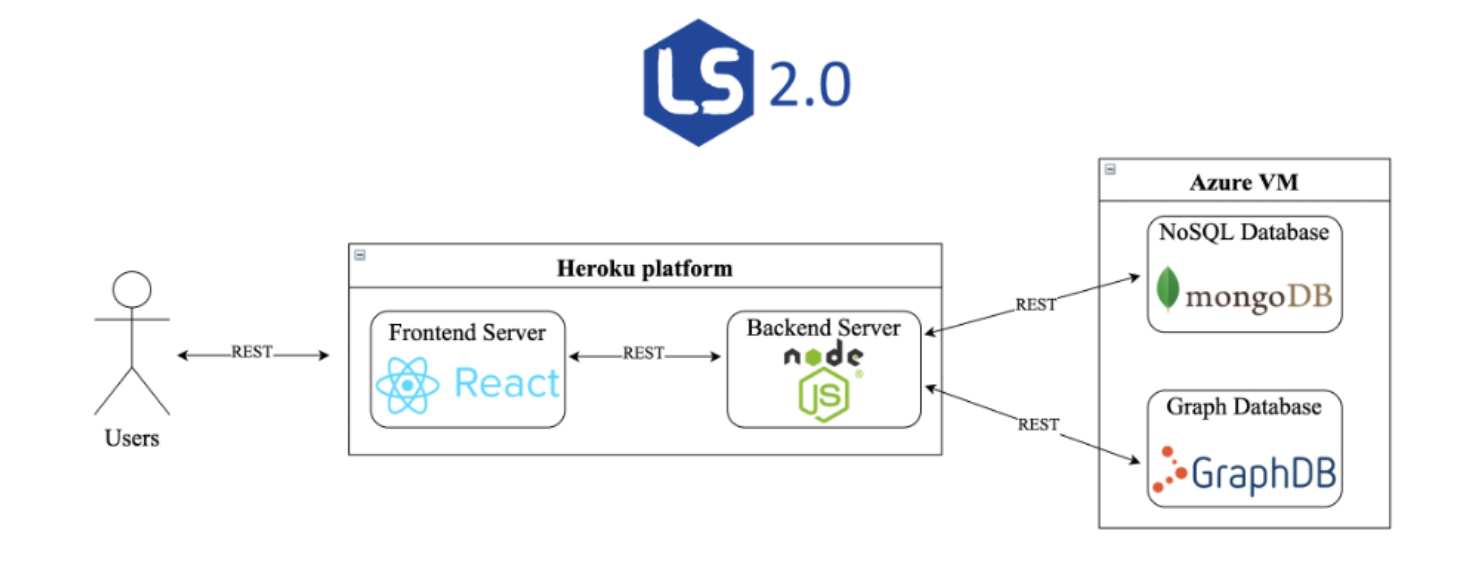
\includegraphics[width=0.8\textwidth]{images/LS2Architecture.png}
  \caption{LS2.0 Technology Stack. Source: Lopes~\cite{lopes_ontologies_2021}.}
  \label{fig:ls2_arch}
\end{figure}

While this architecture demonstrated scalabilty, modularity and adherence to
modern web development practices, it presented several critical limitations,
mainly in the fact that it is not integrated with the ISCTE Moodle environment
(FR2), relying on manual input by the faculty and students making it not an
ideal system and one that would become more of a chore for teachers who have
most commonly multiple classes to teach, register and manage and students who
also have multiple classes, quizes and exercises to keep track of.

We must then conjure a system that is integrated with the ISCTE moodle
environment and satisfies all functional and non-functional requirements set
previously.

At first glance, it is possible to achieve a more integrated system making use
of the platform developed previously with the use of the moodle native web
services, although the standalone nature necessitated separate authentication
systems, creating friction for users who must maintain multiple credentials and
navigate between distinct platforms. The external infrastructure dependencies
resulted in ongoing operational costs, particularly following Heroku's
discontinuation of free tier services~\cite{heroku_pricing}, and introduced
security vulnerabilities through external data hosting that may not align with
institutional data governance policies.

\subsection{Plugin-Based Architecture Benefits}
\noindent The Learning Scorecard 2.5 plugin-based architecture approach addresses these limitations through direct integration with Moodle's comprehensive infrastructure and Service API ecosystem. This approach provides several critical advantages that enhance both technical capabilities and institutional viability.

\textit{Infrastructure Integration} By operating within Moodle's establish infrastructure, LS 2.5 eliminates external hsting requirements and associated costs while ensuring compliance with institutional security and data governance policies. The platform leverages existing ISCTE server infrastructure, Apache web servers and database systems without requiring additional resources or maintenance overhead.

\textit{Authentication and User Management} Integration with Moodle's authentication system erases the need for separate user credentials and login processes, reducing friction for students and faculty while ensuring consistency with institutional access policies. The platform automatically inherits Moodle's sophisticated role and permission systems, enabling fine-grained access control without additional implemenetation complexity.

\textit{Data Ecosystem Access} Perhaps most critically, the plugin arhitecture provides direct access to Moodle's comprehensive student activity and performance data, enabling automated data collection and real-time analytics without manual input requirements. This access includes quiz results, assignment submissions, forum participation, resource access patterns and completion tracking data that can be seamlessly integrated into gamification and analytics workflows.

\textit{User Experience Consistency} The plugin approach ensures visual and functional consistency with existing institutional interfaces, reducing learning curves for users and promoting adoption through familiar interaction patterns. Students and faculty can access Learning Scorecard fuctionality without leaving their established academic workflows.

\subsection{Concept Mapping \& Integration Analysis}

The successful integration of Learning Scorecard functionality within Moodle's
existing architecture requires comprehensive analysis of conceptial alignments
and implementation feasibilities. This mapping process identifies opportunities
for leveraging existing Moodle capabilities while determining areas that
require custom implementation to preserve Learning Scorecard legacy features.

\begin{center}
  \captionof{table}{Learning Scorecard vs Moodle Concept Mapping}
  \begin{tabular}{ccc}
    Concept            & Moodle                               & Feasibility \\ \hline
    \multicolumn{3}{c}{\textit{Academic}}                                   \\
    Course             & Course Categories                    & T           \\
    Curricular Unit    & Course                               & T           \\
    Student            & Users \& Roles                       & T           \\
    Teacher / Faculty  & Users \& Roles                       & T           \\
    Syllabus Contents  & Course Modules \& Tags               & T           \\
    Calendar           & Calendar Events                      & P           \\
    Timeline           & Activity Completion \& Progress      & P           \\
    \multicolumn{3}{c}{\textit{Gamification}}                               \\
    Experience Points  & Grade Items \& Custom Fields         & P           \\
    Ranks              & Custom Implementation                & P           \\
    Quests             & Activities                           & T           \\
    Alliances          & Groups \& Cohorts                    & T           \\
    Guilds             & Groups                               & T           \\
    Badges             & Badges System                        & T           \\
    Trophies           & Badges System \& Custom Impl.        & P           \\
    Avatars            & User Profiles, Files \& Custom Impl. & P           \\
    Leaderboards       & Gradebook \& Custom Views            & P           \\
    Last Chance System & Conditional Activities               & P
  \end{tabular}
  \caption*{T - Total Mapping  P - Partial Mapping}
\end{center}

\section{Development Environment and Technical Infrastructure}
\noindent The establishment of a robust, consistent and production-like development environment proved critical for the successful implementation of LS 2.5. The complexity of Moodle plugin development, combined with the need for the system to mimick the production environment as much as possible, required careful consideration of development infrastructure and tooling decisions.

\subsection{Development Environment Evolution}
\noindent The development environment configuration process revealed important insights into the requirements and challenges of Moodle plugin development, ultimately leading to the identification of optimal approaches for maintaining development productivity and most importantly, system reliability.

The initial development approach employed XAMPP~\cite{apache_friends_xampp} to
provide a local PHP environment, apache server and Mysql database
infrastructure, imperative for standalone Moodle instance execution. However,
this approach demonstrated significant limitation that compromised development
reliability and consistency. File persistence issues following server restarts
and unpredicatable system behavior created an unstable foundation that was
incompatible with the production-like development environment required for
plugin implementation.

The second development approach investigated Docker
containerization~\cite{docker_containers} with orchestrated Bitnami Moodle
image~\cite{bitnami_cloud} to achieve improved consistency and reproducibility.
While this approach initially showed promise through improved container
persistence and more predictable behavier, plugin integration revealed critical
limitations. The Bitnami image implemented included automated Moodle
configuration processes that incorrectly identified plugin additions as
corrupted system files, triggering unwanted fresh installations that
compromised the continuity of the plugin's development and was therefore
excluded from consideration for the final Moodle development environment.

The final development environment employed custom docker container
orchestration with separate Apache server and MariaDB
database~\cite{mariadb_database} images, enabling manual Moodle configuration
that avoided the automated configuration issues encountered with pre-built
images (like Bitnami's). Although with the increased effort of configuring the
apache server and installing the same Moodle version as the production ISCTE
2024/2025 Moodle instance (version 4.4.1) and all the necessary dependencies
this approach provided the stability, consistency and production-like behavior
expected and required for reliable plugin development.

\section{Plugin Integration with Moodle}
\noindent There are multiple types of moodle plugins and depending on their purpose we should select the most adequate. According to the specification of the Learning Scorecard we would need to evaluate what plugin type is better suited.

Moodle's comprehensive plugin architecture~\cite{moodle_plugin_api} provides
multiple plugin types, each optimized for specific functionality categories and
integration patterns. The Learning Scorecard implementation requirements
necessitated evaluation of plugin types to ensure appropriate functionality
distribution and optimal integration with Moodle's existing systems.

Block plugins emerged as the optimal choice for user-facing dashboard and
metric displays. The block architecure's deisgn for small, configurable
information displays that can be positioned throughout Moodle's interface
aligns perfectly with Learning Scorecard's requirement for accessible
gamification metrics within existing workflows. block plugins enable experience
point displays, ranking information and progress metrics to be seamlessly
integrated into student and faculty dashboards without requiring navigation to
separate interfaces.

Local plugins generic specification provide the appropriate architecture for
additional LS functionality, including leaderboards, Learning Scorecard
configuration, database table creation, etc.

The modular plugin approach requires appropriate directory organization within
Moodle's established file structure. Block plugins are installed within the
\textit{"/blocks"} directory, while local plugins reside in the
\textit{"/local"} directory, ensuring compliance with Moodle's architectural
standards and enabling proper plugin discovery and management through Moodle's
administrative interfaces.

\section{Database Design and Data Integration}

\chapter{MVP}
\section{System Components and Modular Design}
\subsection{Student Interface and Experience}
\subsection{Teacher Dashboard and Analytics}
\subsection{Administrator Functions and Control}

\chapter{Evaluation and Results}
\section{Demonstration of Key Features}
\section{Feedback and Empirical Results}
\section{Comparative Analysis with Previous Approaches}
\section{Discussion of Evaluation Metrics}

\chapter{Conclusions}
\section{Summary of Contributions}
\section{Limitations and Challenges}
\section{Future Directions for LS}

\renewcommand{\bibname}{References}

\def\bibindent{0.7cm}
\begin{thebibliography}{99\kern\bibindent}
  \makeatletter
  \let\old@biblabel\@biblabel
  \def\@biblabel#1{\old@biblabel{#1}\kern\bibindent}
  \let\old@bibitem\bibitem
  \def\bibitem#1{\old@bibitem{#1}\leavevmode\kern-\bibindent}
  \makeatother
  \makeatletter
  \renewcommand\@biblabel[1]{}
  \makeatother

  \bibitem{deterding_gamification_2011} S. Deterding, R. Khaled, L. Nacke and D. Dixon (2011), \textquotedblleft Gamification: Toward a definition\textquotedblright, \textit{Proceedings of CHI 2011 Workshop Gamification: Using Game Design Elements in Non-Game Contexts}, 6--9.

  \bibitem{mohd_kasim_choosing_2016} N.N. Mohd Kasim and F. Khalid (2016), \textquotedblleft Choosing the Right Learning Management System (LMS) for the Higher Education Institution Context: A Systematic Review\textquotedblright, \textit{International Journal of Emerging Technologies in Learning (iJET)}, 11(6), 55.

  \bibitem{cavus_comparison_2014} N. Cavus and T. Zabadi (2014), \textquotedblleft A Comparison of Open Source Learning Management Systems\textquotedblright, \textit{Procedia - Social and Behavioral Sciences}, 143, 521--526.

  \bibitem{altinpulluk_systematic_2021} H. Altinpulluk and M. Kesim (2021), \textquotedblleft A Systematic Review of the Tendencies in the Use of Learning Management Systems\textquotedblright, \textit{Turkish Online Journal of Distance Education}, 22(3), 40--54.

  \bibitem{moodle_stats_2025} Moodle (2025), \textquotedblleft Moodle Statistics\textquotedblright, Available at: https://stats.moodle.org/ (Accessed: 6 August 2025).

  \bibitem{dolawattha_impact_2019} D.D.M. Dolawattha, H.K.S. Pramadasa and P.M. Jayaweera (2019), \textquotedblleft The Impact Model: Teachers' Mobile Learning Adoption in Higher Education\textquotedblright, \textit{International Journal of Education and Development using Information and Communication Technology (IJEDICT)}, 15(4), 71--88.

  \bibitem{saroja_functional_2023} S. Saroja and S. Haseena (2023), \textquotedblleft Functional and Non-Functional Requirements in Agile Software Development\textquotedblright, in \textit{Agile Software Development}, John Wiley \& Sons, Ltd, pp. 71--86.

  \bibitem{costa_thesis_2017} D.S. Costa (2017), \textquotedblleft Learning Scorecard: Plataforma para a Monitorização da Experiência de Aprendizagem de Alunos no Ensino Superior Aplicando Técnicas de Business Intelligence e Gamificação\textquotedblright, Master's Thesis, ISCTE-IUL, Lisbon, Portugal.

  \bibitem{react_dev} Meta Platforms, Inc. (2024), \textquotedblleft React: The Library for Web and Native User Interfaces\textquotedblright, Available at: https://react.dev/ (Accessed: 28 August 2025).

  \bibitem{express_js} OpenJS Foundation (2024), \textquotedblleft Express: Fast, Unopinionated, Minimalist Web Framework for Node.js\textquotedblright, Available at: https://expressjs.com/ (Accessed: 28 August 2025).

  \bibitem{nodejs_org} OpenJS Foundation (2024), \textquotedblleft Node.js: JavaScript Runtime Built on Chrome's V8 JavaScript Engine\textquotedblright, Available at: https://nodejs.org/en/ (Accessed: 28 August 2025).

  \bibitem{azure_microsoft} Microsoft Corporation (2024), \textquotedblleft Microsoft Azure: Cloud Computing Platform and Services\textquotedblright, Available at: https://azure.microsoft.com/en-us/ (Accessed: 28 August 2025).

  \bibitem{mongodb_database} MongoDB, Inc. (2024), \textquotedblleft MongoDB: The Developer Data Platform\textquotedblright, Available at: https://www.mongodb.com/ (Accessed: 28 August 2025).

  \bibitem{graphdb_ontotext} Ontotext (2024), \textquotedblleft GraphDB: Enterprise Ready RDF Database\textquotedblright, Available at: https://graphdb.ontotext.com/ (Accessed: 28 August 2025).

  \bibitem{heroku_platform} Salesforce, Inc. (2024), \textquotedblleft Heroku: Cloud Application Platform\textquotedblright, Available at: https://www.heroku.com/ (Accessed: 28 August 2025).

  \bibitem{lopes_ontologies_2021} M.Â.D. Lopes (2021), \textquotedblleft Utilização de ontologias para a gestão de dados educacionais: caso de estudo Learning Scorecard\textquotedblright, Master's Thesis, ISCTE - Instituto Universitário de Lisboa, Lisbon, Portugal.

  \bibitem{heroku_pricing} Salesforce, Inc. (2024), \textquotedblleft Heroku Pricing\textquotedblright, Available at: https://www.heroku.com/pricing/ (Accessed: 28 August 2025).

  \bibitem{git_scm} Git Community (2024), \textquotedblleft Git: Distributed Version Control System\textquotedblright, Available at: https://git-scm.com/.

  \bibitem{apache_friends_xampp} Apache Friends (2024), \textquotedblleft XAMPP Apache + MariaDB + PHP + Perl\textquotedblright, Available at: https://www.apachefriends.org/.

  \bibitem{docker_containers} Docker Inc. (2024), \textquotedblleft Docker: Accelerated Container Application Development\textquotedblright, Available at: https://www.docker.com/.

  \bibitem{bitnami_cloud} Bitnami (2024), \textquotedblleft Bitnami: Packaged Applications for Any Platform\textquotedblright, Available at: https://bitnami.com/.

  \bibitem{mariadb_database} MariaDB Foundation (2024), \textquotedblleft MariaDB Server: The Open Source Relational Database\textquotedblright, Available at: https://mariadb.org/.

  \bibitem{moodle_plugin_api} Moodle Pty Ltd (2024), \textquotedblleft Plugin Types API Documentation\textquotedblright, Moodle Developer Resources, Available at: https://moodledev.io/docs/4.1/apis/plugintypes.
\end{thebibliography}

\end{document}
